%4619055 課題4
\documentclass[12pt]{jarticle}
\usepackage{TUSIreport}
\usepackage{otf}
\usepackage[dvipdfmx]{graphicx}
\usepackage{amsmath}
\usepackage{amssymb}
\usepackage{hhline}
\usepackage{fancybox,ascmac}
\usepackage{url}
\usepackage{multirow}
%%%%%%%%%%%%%%%%%%
\begin{document}
%%%%%%%%%%%%%%%%%%%%%%%%%%%%%%%%%%%%%%%%%%%%%%%%%%%%%%%%
% 表紙を出力する場合は,\提出者と\共同実験者をいれる
% \提出者{科目名}{課題名}{提出年}{提出月}{提出日}{学籍番号}{氏名}
% \共同実験者{一人目}{二人目}{..}{..}{..}{..}{..}{八人目}
%%%%%%%%%%%%%%%%%%%%%%%%%%%%%%%%%%%%%%%%%%%%%%%%%%%%%%%
\提出者{情報工学実験1}{課題4 統計学入門}
{2020}{8}{3}{4619055}{辰川力駆}

\共同実験者{}{}{}{}{}{}{}{}
\追加実験者{}{}
\表紙出力

\section{実験の目的}
\begin{itemize}
    \item[(1)] 離散分布の理解

          代表的な離散分布である二項分布を理解する。
    \item[(2)]標本平均の分布

          中心極限定理を理解する。
    \item[(3)] 連続分布の理解

          代表的な連続分布である正規分布を理解する。
\end{itemize}

\section{実験1}
二項分布を基にした実験

\subsection{目標}
離散分布の基本として二項分布の特徴を理解する。
\subsection{実験手順}
\begin{itemize}
    \item[(1)] ``赤4個、白6個の合計10個の玉が入った箱から1つ取り出して色を確認後、
          取り出した玉を箱に戻す作業を5回繰り返す。"
          というのを1回の試行として、これを30回試行して記録する。
    \item[(2)] 取り出された赤玉の回数の度数表と棒グラフをExcelで作成する。
    \item[(3)] 取り出された赤玉の個数の平均値を求める。
\end{itemize}
\subsection{実験結果}
以下に実験結果の表とグラフを示す。
また、取り出された赤玉の個数の平均値は約2.433333333となった。

\clearpage
\begin{table}
    \begin{center}
        \caption{試行における赤玉の個数}
        \begin{tabular}[h]{|c|c|c|c|c|c|c|}
            \hline
            \multirow{2}{*}{試行} & \multicolumn{5}{|c|}{回数} & \multirow{2}{*}{赤玉の個数}                    \\
            \cline{2-6}
                                  & 1                          & 2                           & 3  & 4  & 5  &   \\
            \hline
            1                     & 〇                         & 〇                          & 〇 & ×  & 〇 & 4 \\
            2                     & ×                          & 〇                          & ×  & 〇 & ×  & 2 \\
            3                     & 〇                         & ×                           & 〇 & 〇 & ×  & 3 \\
            4                     & ×                          & 〇                          & ×  & ×  & 〇 & 2 \\
            5                     & ×                          & ×                           & 〇 & 〇 & ×  & 2 \\
            6                     & 〇                         & ×                           & 〇 & ×  & ×  & 2 \\
            7                     & 〇                         & ×                           & 〇 & ×  & 〇 & 3 \\
            8                     & 〇                         & ×                           & 〇 & 〇 & 〇 & 4 \\
            9                     & ×                          & ×                           & ×  & 〇 & ×  & 1 \\
            10                    & ×                          & ×                           & 〇 & ×  & ×  & 1 \\
            11                    & ×                          & 〇                          & ×  & ×  & 〇 & 2 \\
            12                    & ×                          & 〇                          & 〇 & 〇 & ×  & 3 \\
            13                    & 〇                         & 〇                          & 〇 & 〇 & ×  & 4 \\
            14                    & 〇                         & 〇                          & ×  & 〇 & ×  & 3 \\
            15                    & 〇                         & 〇                          & 〇 & ×  & ×  & 3 \\
            16                    & 〇                         & ×                           & 〇 & 〇 & 〇 & 4 \\
            17                    & ×                          & ×                           & ×  & ×  & ×  & 0 \\
            18                    & ×                          & ×                           & ×  & 〇 & 〇 & 2 \\
            19                    & 〇                         & ×                           & ×  & 〇 & 〇 & 3 \\
            20                    & 〇                         & ×                           & 〇 & 〇 & ×  & 3 \\
            21                    & ×                          & 〇                          & 〇 & ×  & 〇 & 3 \\
            22                    & 〇                         & ×                           & ×  & ×  & ×  & 1 \\
            23                    & ×                          & ×                           & ×  & ×  & 〇 & 1 \\
            24                    & ×                          & 〇                          & 〇 & 〇 & 〇 & 4 \\
            25                    & ×                          & ×                           & 〇 & 〇 & 〇 & 3 \\
            26                    & 〇                         & ×                           & ×  & ×  & 〇 & 2 \\
            27                    & 〇                         & ×                           & 〇 & ×  & ×  & 2 \\
            28                    & 〇                         & 〇                          & ×  & 〇 & 〇 & 4 \\
            29                    & 〇                         & ×                           & ×  & ×  & ×  & 1 \\
            30                    & ×                          & ×                           & 〇 & ×  & ×  & 1 \\
            \hline
                                  & \multicolumn{5}{|c|}{平均} & 2.433333333                                    \\
            \hline
        \end{tabular}
    \end{center}
\end{table}
\clearpage

\begin{table}
    \begin{center}
        \caption{出現回数の度数表}
        \begin{tabular}[h]{|c|c|}
            \hline
            赤玉の個数 & 度数 \\
            \hline
            0          & 1    \\
            1          & 6    \\
            2          & 8    \\
            3          & 9    \\
            4          & 6    \\
            5          & 0    \\
            \hline
        \end{tabular}
    \end{center}
\end{table}
\begin{figure}[h]
    \begin{center}
        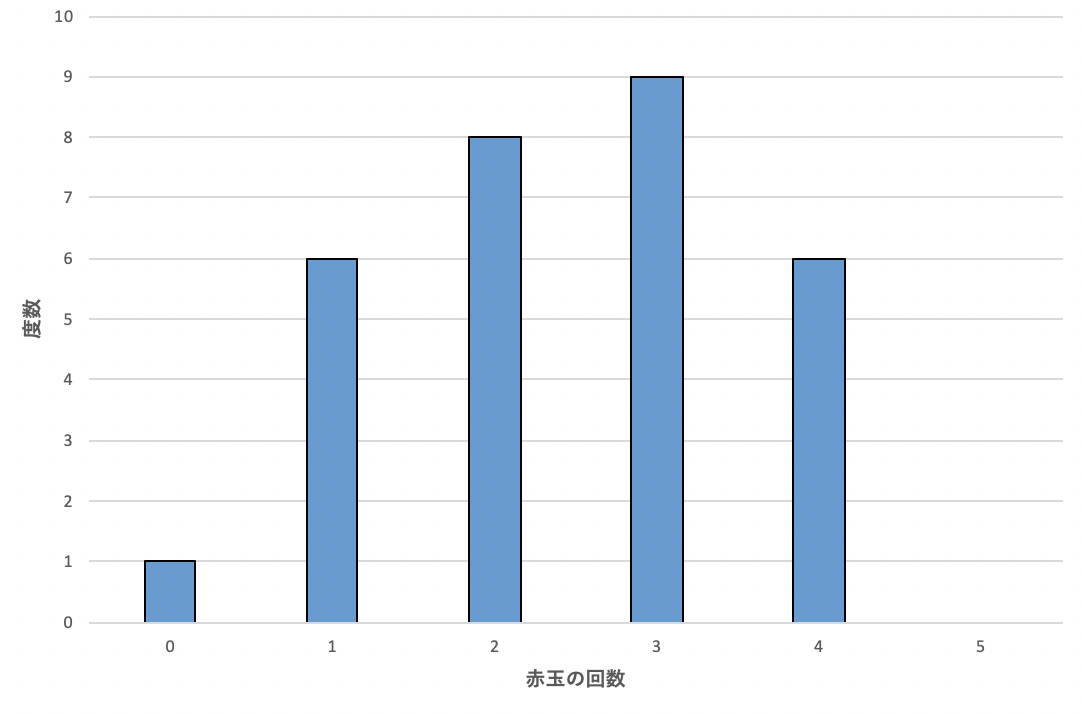
\includegraphics[scale=0.9]{kadai4_1graph1.png}
    \end{center}
    \caption{赤玉出現回数の棒グラフ}
\end{figure}
\clearpage

\subsection{レポート課題}
\subsubsection*{レポート課題1-1}
\begin{shadebox}
    実験1の結果をまとめよ。
\end{shadebox}
表1の実験結果より、平均値は約2.433333333である。
また、表2の度数分布より最頻値は3であり、中央値は2.5である。
ヒストグラムを見ると明らかであるが、0と5の頻度が少ない。
そして1から4はほぼ頻度が同じなので、平均値と中央値がほとんど同じと考えられる。

\subsubsection*{レポート課題1-2}
\begin{shadebox}
    実験1の結果は、二項分布に従っているといえるか述べよ。
\end{shadebox}
実験1の結果は、二項分布に従っていない。

二項分布の公式より
\begin{equation}
    P(X=k)= {}_n C_k p^k{(1-p)}^{n-k} \nonumber
\end{equation}
である。
今回は、条件より$n=5$、$p=0.4$として$k=0,1,2,3,4,5$を計算すると、
\begin{eqnarray}
    P(X=0)= {}_5 C_0 0.4^0{(1-0.4)}^{5-0} \fallingdotseq  0.0778 \nonumber \\
    P(X=1)= {}_5 C_1 0.4^1{(1-0.4)}^{5-1} \fallingdotseq  0.2592 \nonumber \\
    P(X=2)= {}_5 C_2 0.4^2{(1-0.4)}^{5-2} \fallingdotseq 0.3456\nonumber \\
    P(X=3)= {}_5 C_3 0.4^3{(1-0.4)}^{5-3} \fallingdotseq 0.2304 \nonumber \\
    P(X=4)= {}_5 C_4 0.4^4{(1-0.4)}^{5-4} \fallingdotseq 0.0768 \nonumber \\
    P(X=5)= {}_5 C_5 0.4^5{(1-0.4)}^{5-5} \fallingdotseq 0.0102\nonumber
\end{eqnarray}
となるが、実験から出される確率は、
\begin{eqnarray}
    P(X=0) &=& 1÷30 \fallingdotseq 0.3333 \nonumber \\
    P(X=1)&=& 6÷30 = 0.2 \nonumber \\
    P(X=2)&=& 8÷30 \fallingdotseq 0.2667\nonumber \\
    P(X=3)&=& 9÷30 = 0.3 \nonumber \\
    P(X=4)&=& 6÷30 = 0.2 \nonumber \\
    P(X=5)&=& 0÷30 = 0 \nonumber
\end{eqnarray}
となる。これは、二項分布の公式から出した値と一致しない。

したがって、実験1の結果は、二項分布に従っていない。

\clearpage
\section{実験2}
中心極限定理を基にした実験

\subsection{目標}
標本平均の分布について理解する。

\subsection{実験手順}
\begin{itemize}
    \item[(1)] Excelの[データ]から[データ分析]を選び、続いて[乱数発生]を選択する。
    \item[(2)] 0から1までの1000個の乱数を発生させる。
    \item[(3)] 発生させた乱数のヒストグラムを作成する。
    \item[(4)] 区間幅を0.01としてヒストグラムを作成する。
    \item[(5)] 0から1までの1000個の乱数を2つ発生させ、その平均値のヒストグラムを作成する。
    \item[(6)] 0から1までの1000個の乱数を8つ発生させ、その平均値のヒストグラムを作成する。
    \item[(7)] 0から1までの1000個の乱数を100つ発生させ、その平均値のヒストグラムを作成する。
\end{itemize}

\subsection{実験結果}
以下に実験結果のグラフを示す。

\begin{figure}[h]
    \begin{center}
        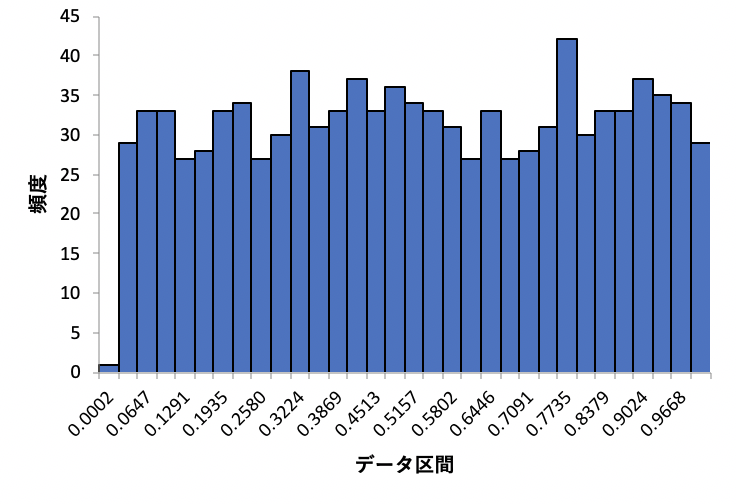
\includegraphics[scale=0.8]{kadai4_2graph1.png}
    \end{center}
    \caption{1000個の乱数を発生させた結果のヒストグラム(変数1つの区間幅指定なし)}
\end{figure}
\begin{figure}[h]
    \begin{center}
        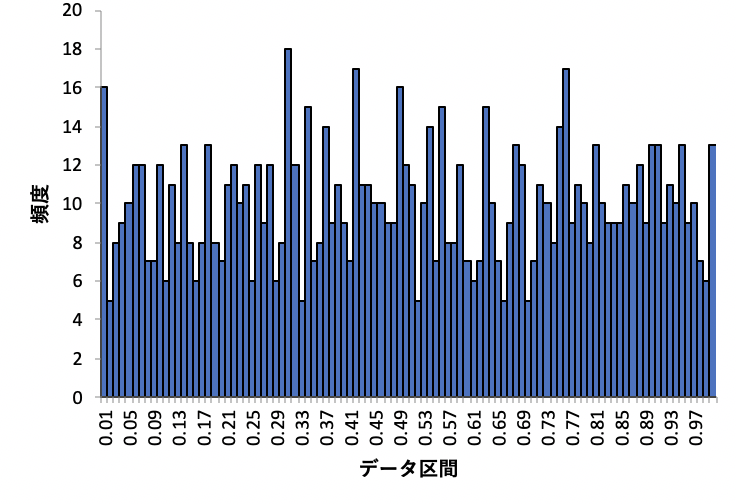
\includegraphics[scale=0.8]{kadai4_2graph2.png}
    \end{center}
    \caption{1000個の乱数を発生させた結果のヒストグラム(変数1つ)}
\end{figure}
\begin{figure}[h]
    \begin{center}
        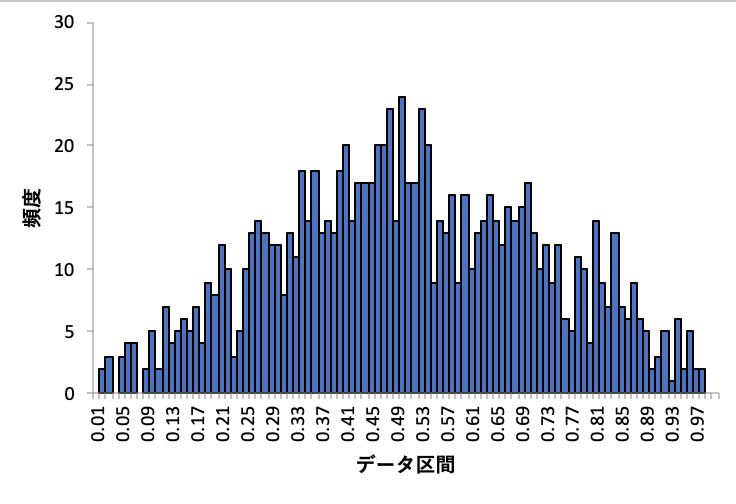
\includegraphics[scale=0.8]{kadai4_2graph3.png}
    \end{center}
    \caption{1000個の乱数を発生させた結果の平均値のヒストグラム(変数2つ)}
\end{figure}
\begin{figure}[h]
    \begin{center}
        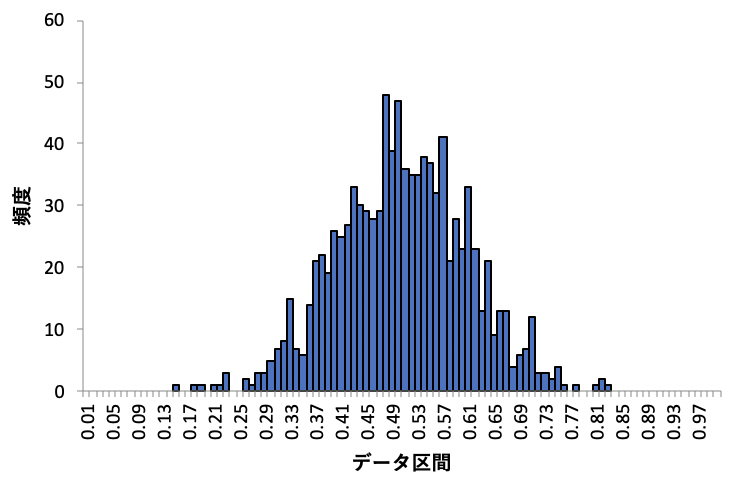
\includegraphics[scale=0.8]{kadai4_2graph4.png}
    \end{center}
    \caption{1000個の乱数を発生させた結果の平均値のヒストグラム(変数8つ)}
\end{figure}
\begin{figure}[h]
    \begin{center}
        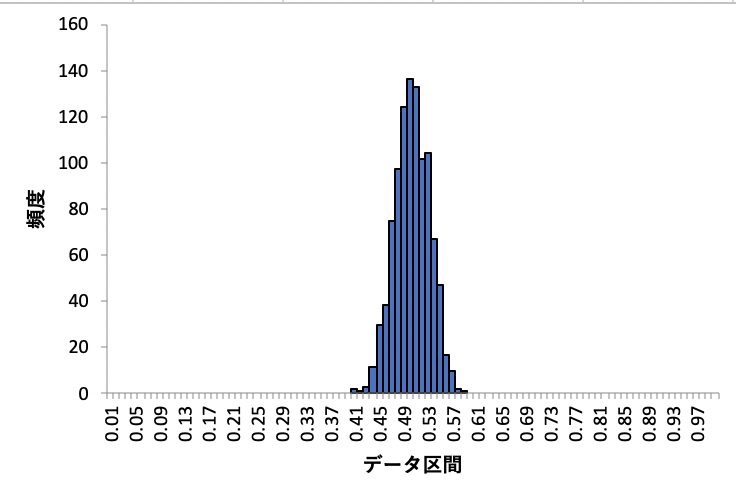
\includegraphics[scale=0.8]{kadai4_2graph5.png}
    \end{center}
    \caption{1000個の乱数を発生させた結果の平均値のヒストグラム(変数100つ)}
\end{figure}

\clearpage

\subsection{レポート課題}
\subsubsection*{レポート課題2-1}
\begin{shadebox}
    実験2の結果をまとめよ。
\end{shadebox}
それぞれの図より、変数の数を増加させるとデータが中央に寄った。
今回の場合は0から1までの乱数を1000個作ったので0.5に寄ったことになる。
また、変数の数を更に大きくすると、さらに中央に寄ると考えられる。

\subsubsection*{レポート課題2-2}
\begin{shadebox}
    大数の法則とは何か、実験2の結果に基づいて説明せよ。
\end{shadebox}
大数の法則とは、確率$p$で起こる事象において、試行回数を増やすほど、
その事象が実際に起こる確率は$p$に近づくという法則である。

今回はExcel上で均一分布で乱数を発生させたので、
無限個の母集団の平均値は範囲の中央の値になる。
従って0.5に寄ることになるが、レポート課題2-1でも述べたように変数の数を大きくするにつれて0.5に寄っている。

\subsubsection*{レポート課題2-3}
\begin{shadebox}
    中心極限定理とは何か、実験2の結果に基づいて説明せよ。
\end{shadebox}
中心極限定理とは、標本を抽出する母集団が平均$\mu$、
分散$ \sigma^2$の正規分布に従う従わないに関わらず、
抽出するサンプルサイズ$n$が大きくなるにつれて標本平均の分布は「平均$\mu$、分散$\frac{\sigma^2}{n}$」の
正規分布 $N$($\mu$,$\frac{\sigma^2}{n}$) に近づくという定理である。
実際、今回の実験で変数の数を大きくするにつれてグラフの概形が正規分布に近づいている。

\subsubsection*{レポート課題2-4}
\begin{shadebox}
    区間 [0,1] の一様分布から12個選び、その合計から6を引いた値をYとする。
    Y はどのような分布に従うか述べよ。
\end{shadebox}
区間 [0,1] の一様分布から12個選ぶので、
分散と平均は元の一様分布に従う。
したがって、Y は正規分布に近づくと考えられる。

\clearpage

\section{実験3}
正規分布を基にした実験

\subsection{目標}
正規分布の概要について理解する。

\subsection{実験手順}
\begin{itemize}
    \item[(1)] Excelの[データ]から[データ分析]を選び、続いて[乱数発生]を選択する。
    \item[(2)] 0から1までの1000個の乱数を平均を0、標準偏差を1として正規分布に従って発生させる。
    \item[(3)] [データ区間]に指定する数値(区間幅0.5刻みの-10から10)を作る。
    \item[(4)] ヒストグラムを作成する。
    \item[(5)] 同様の手順で、平均を変更した場合に発生する乱数を用いてヒストグラムを作成する。
          \begin{itemize}
              \item 平均 -2、標準偏差 1
              \item 平均 2、標準偏差 1
          \end{itemize}
    \item[(6)] 同様の手順で、標準偏差を変更した場合に発生する乱数を用いてヒストグラムを作成する。
          \begin{itemize}
              \item 平均 0、標準偏差 2
              \item 平均 0、標準偏差 4
          \end{itemize}
\end{itemize}

\subsection{実験結果}
以下に実験結果のグラフを示す。

\begin{figure}[h]
    \begin{center}
        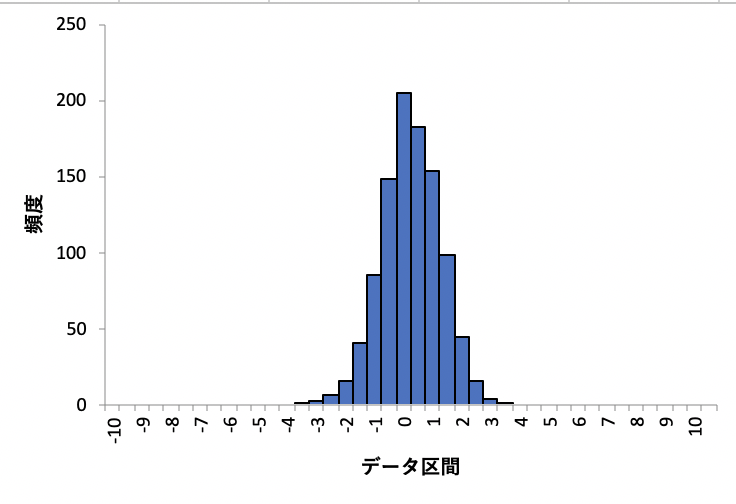
\includegraphics[scale=0.6]{kadai4_3graph1.png}
    \end{center}
    \caption{平均が0、標準偏差が1の乱数を発生させた結果のヒストグラム}
\end{figure}

\clearpage
\begin{figure}[h]
    \begin{center}
        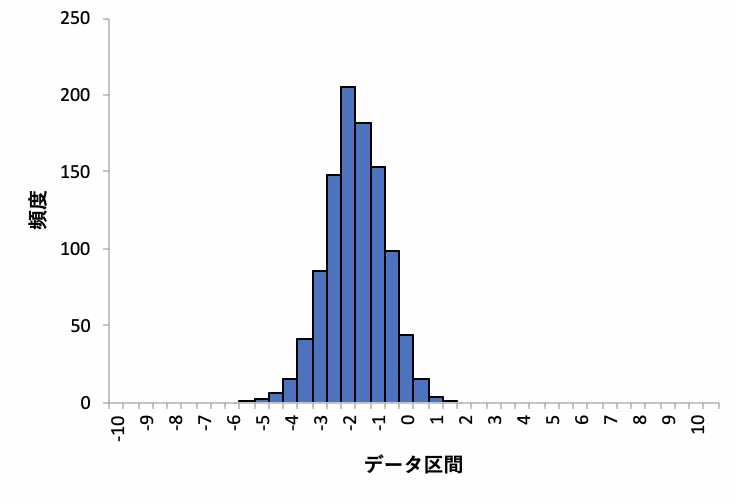
\includegraphics[scale=0.7]{kadai4_3graph2.png}
    \end{center}
    \caption{平均が-2、標準偏差が1の乱数を発生させた結果のヒストグラム}
\end{figure}
\begin{figure}[h]
    \begin{center}
        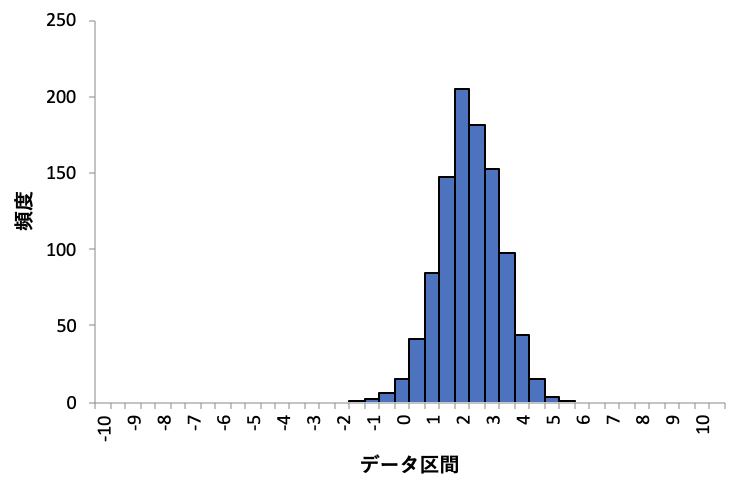
\includegraphics[scale=0.7]{kadai4_3graph3.png}
    \end{center}
    \caption{平均が2、標準偏差が1の乱数を発生させた結果のヒストグラム}
\end{figure}
\clearpage

\begin{figure}[h]
    \begin{center}
        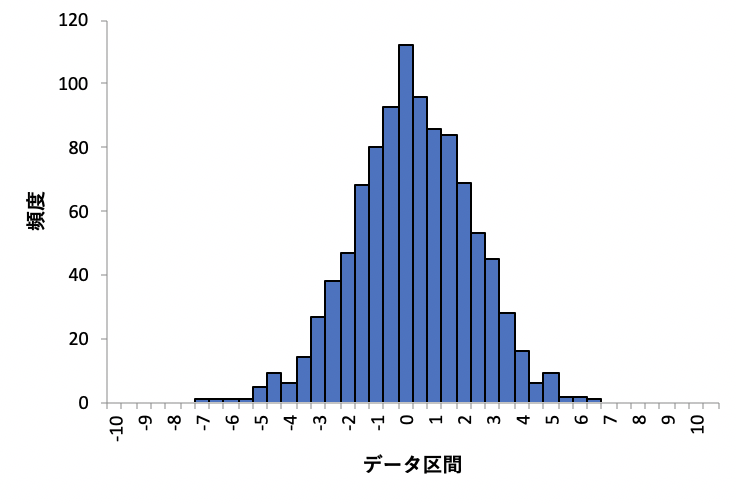
\includegraphics[scale=0.7]{kadai4_3graph4.png}
    \end{center}
    \caption{平均が0、標準偏差が2の乱数を発生させた結果のヒストグラム}
\end{figure}
\begin{figure}[h]
    \begin{center}
        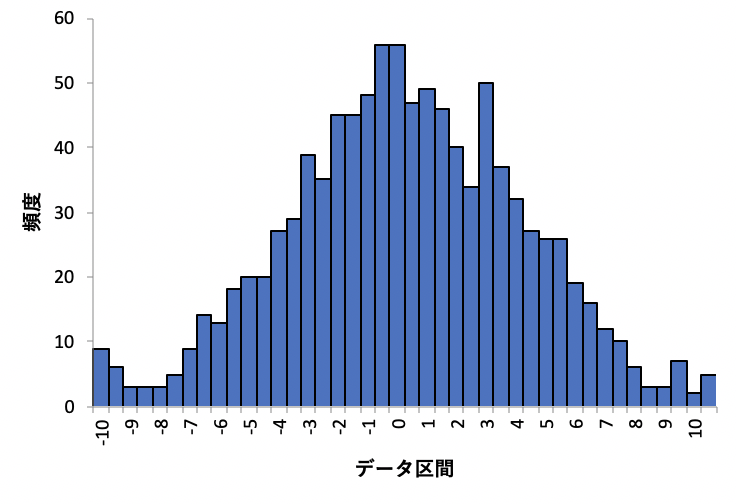
\includegraphics[scale=0.7]{kadai4_3graph5.png}
    \end{center}
    \caption{平均が0、標準偏差が4の乱数を発生させた結果のヒストグラム}
\end{figure}
\clearpage

\subsection{レポート課題}
\subsubsection*{レポート課題3-1}
\begin{shadebox}
    実験3-4、3-5で作成したヒストグラムを比較して、考察せよ。
\end{shadebox}

図7、8、9を比べてみると、
グラフの概形は変わらないが山なりなグラフの場所が移動していることがわかる。
また、その山なりな概形の中心は平均値に一致している。
したがって、図8は図7のグラフに-2、図9は図7のグラフに+2したグラフの概形と考えられる。
よって、乱数を生成する時に標準偏差を一定にしたままで平均値を変更すると、
その平均値の値だけヒストグラムは移動することが分かる。

\subsubsection*{レポート課題3-2}
\begin{shadebox}
    実験3-4、3-6で作成したヒストグラムを比較して、考察せよ。
\end{shadebox}

図7、10、11を比べてみると、
山なりな概形の中心は変わっていないが、
標準偏差を大きくすることによりデータのばらつきが大きくなっている。
また、縦軸のラベルを見ると分かるが、標準偏差を大きくすると同じ数字があまり存在しなくなっている。
よって、乱数を生成する時に平均値を一定にしたままで標準偏差を増やすと、
データのばらつきが大きくなることが分かる。

\subsubsection*{レポート課題3-3}
\begin{shadebox}
    課題3-1、3-2から、
    正規分布における期待値と標準偏差は確率分布の何を決定しているといえるか述べよ。
\end{shadebox}

正規分布において、
期待値は確率分布における平均値を決定している。
また、正規分布における標準偏差は確率分布のデータのばらつきを決定している。

\subsubsection*{レポート課題3-4}
\begin{shadebox}
    偏差値の確率密度関数を書け。
\end{shadebox}

正規分布である確率密度関数$f(x)$は、平均を$\mu$、標準偏差を$\sigma$とすると次のようになる。
\begin{eqnarray}
    f(x)=\frac{1}{\sqrt{2\pi}\sigma}exp\left(-\frac{(x-\mu)^2}{2\sigma^2}\right)
\end{eqnarray}
ここで、偏差値は平均を$\mu=50$、標準偏差を$\sigma=10$としたものであるから、式(1)に代入して
\begin{eqnarray*}
    f(x)=\frac{1}{10\sqrt{2\pi}}exp\left(-\frac{(x-50)^2}{200}\right)
\end{eqnarray*}
となる。

\clearpage
\subsubsection*{レポート課題3-5}
\begin{shadebox}
    試験の点数や順位と比較して偏差値の短所・長所を述べよ。
\end{shadebox}
偏差値は、平均値と標準偏差が決められているので、
平均値や標準偏差が異なる試験においても比較ができるようになっている。

しかし、偏差値は母集団のどのくらいの位置にいるのかが分かるものなので、
母集団が変化した時に偏差値だけでは試験の実力差が分からない。
したがって、母集団が違うもの同士で比較はできない。

\section{結論}
実験を通して、代表的な離散分布である二項分布、標本平均の分布、代表的な連続分布である正規分布を理解した。
また、考察で実験値は二項分布に従っているかどうかや、
標本平均の分布が中心極限定理に従っているかどうかを考えた。

\section{感想}
今回の実験で様々なヒストグラムを比べたので、ヒストグラムについての細かい違いを理解することができた。
また、確率密度関数の使い方について知ることができた。

\clearpage
% 参考文献
\begin{thebibliography}{99}
    \label{sannkoubunnkenn_chapter}
    \bibitem[1]{rikadai}東京理科大学工学部情報工学科「情報工学実験1 2020年度」
    (2020/4/6)

    \bibitem[2]{paa}大数の法則1 | 統計学の時間 | 統計WEB

    \url{https://bellcurve.jp/statistics/course/8539.html}

    最終閲覧日:2020/8/5

    \bibitem[3]{pa}中心極限定理1 | 統計学の時間 | 統計WEB

    \url{https://bellcurve.jp/statistics/course/8543.html}

    最終閲覧日:2020/8/5

\end{thebibliography}

\appendix
%%%%%%%%%%%%%%%%%%%%%%%%%%%%%%%%%%%%%%%%%%%%%%%%%%%%%%%
\end{document}
